
\subsection{Product perspective}


\begin{minipage}{\textwidth}
\begin{center}
\begin{center}
White class are dedicated to perform Data4Help service, the other two applications are listed below.
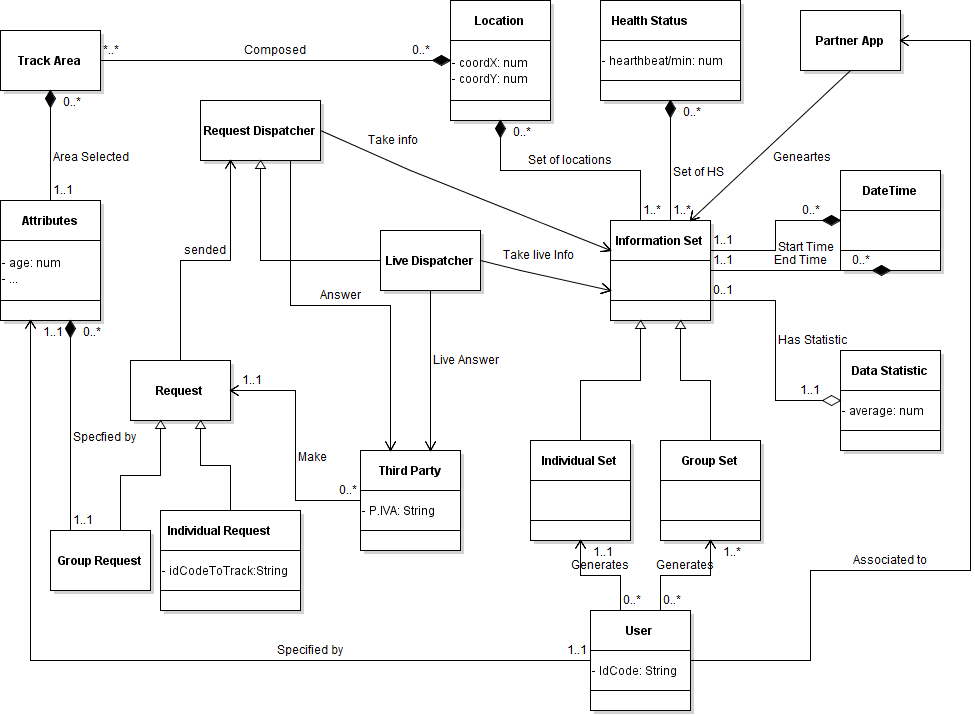
\includegraphics[scale=0.5]{Images/Class_Data4Help.png}
\end{center}
\end{center}

\begin{center}
{\color{Salmon} Red classes} are dedicated to {\color{Salmon} AutomatedSOS} application, supported by Data4Help service (White ones).
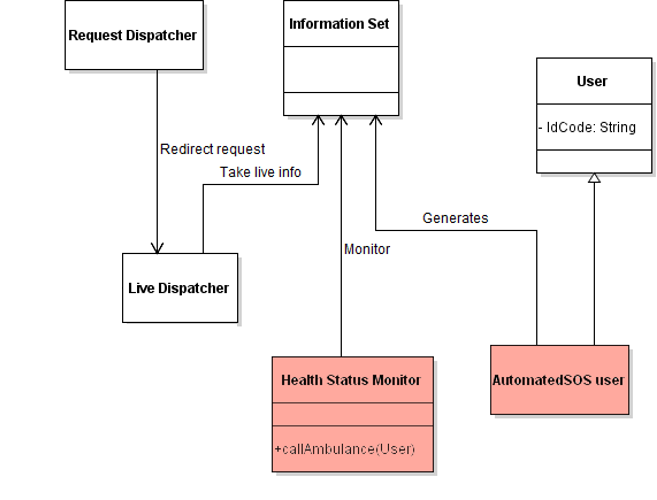
\includegraphics[scale=0.6]{Images/Class_AutoSOS.png}
\end{center}
\end{minipage}

\begin{minipage}{\textwidth}
\begin{center}
{\color{LimeGreen} Green classes} are dedicated to {\color{LimeGreen} Track4Run} application, supported by Data4Help service (White ones).
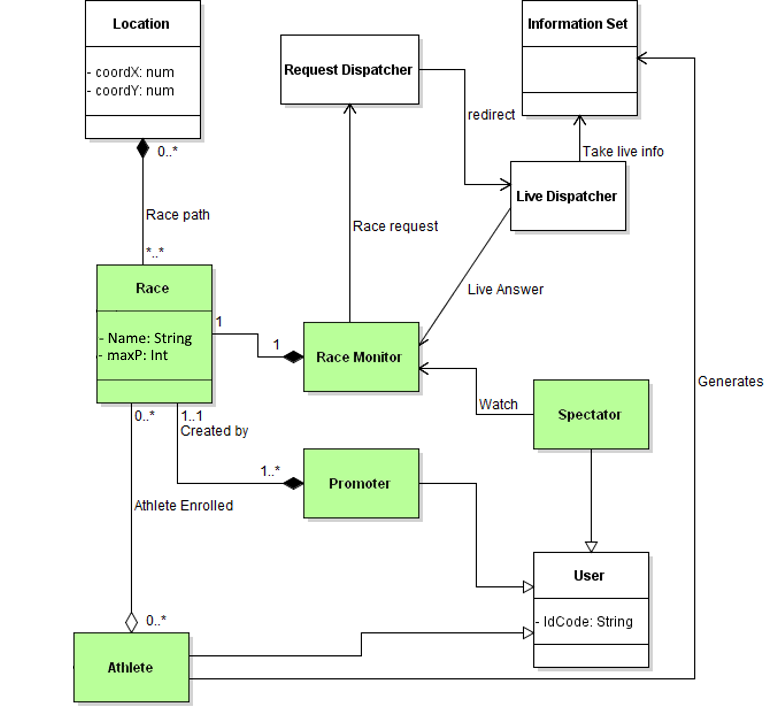
\includegraphics[scale=0.7]{Images/Class_Track4Run.png}
\end{center}
\end{minipage}

\begin{minipage}{\textwidth}
\begin{center}
The following image represent the StateChart of a Request Object.
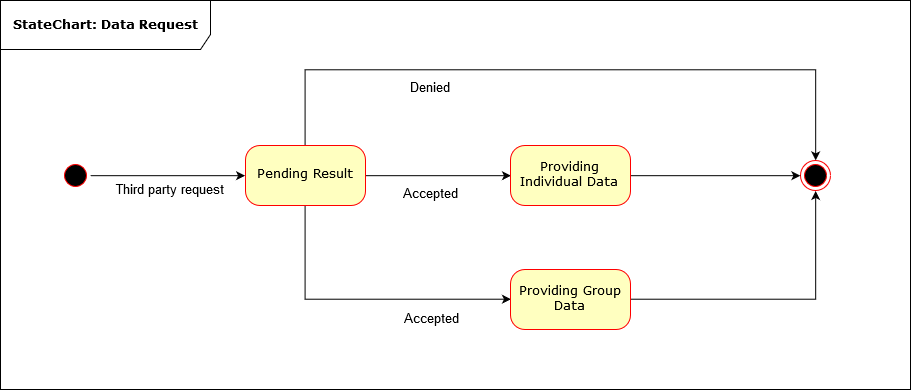
\includegraphics[scale=0.5]{Images/StateChart.png}
\end{center}
\end{minipage}


\subsection{Product functions}
The systems-to-be under analysis have to offer several functions. Below, the main functions provided by each system are more precisely specified, considering all the aspects emerged from the previous list of goals.
\subsubsection{Data4Help - Providing data to third parties }
This is the core function that Data4Help has to ensure. After collecting users position and health status information from external partner applications, Data4Help provides these data to the third party interested in having them. Data4Help provides data on demand sending to the third party all the available data about an individual (or a group of individual) collected so far. So the third party is provided with all the data about a user from the begin to now. In addition, Data4Help offers a providing data service in real time, allowing the third party to subscribe to new data and to receive them as soon as they are produced

\subsubsection{AutomatedSOS - Sending ambulance request in critical situation}
AutomatedSOS monitors the health status of the subscribed customers and, when such parameters are below certain threshold, sends to the location of the customer an ambulance, guaranting a reaction time of less than 5 seconds from the time parameters are below the threshold.
\bigbreak
\noindent
Therefore, the main function offered by AutomatedSOS is sending an ambulance request, with the relative user position, to the near hospital to the user. In order to optimize the times, the ambulance request contains all the data about the user health status. Providing these infomations, when rescures arrive can immediately act accordingly to the alleged anomalous data.
\subsubsection{Track4Run - Run management}
Track4Run offers three different functionaly for its users, which can be all grouped under the 'run management' function. A user can be a promoter, in this case the user can create the event run , which will be visible to every other users. Once created a run, the promoter can define the path in a iteractive way, that is by drawing the path directly on a map. Track4Run allows the promoter to set other additional information, like the start time or an overrall description of the run. Finally, the promoter can invite to the run all the partecipants. 
\bigbreak
\noindent
The atheletes have to be user too. Once recevied a run request, the athlete can enroll the run or reject it. In the first case, Track4Run tracks in real time the partecipant position for all the run through a GPS device. Therefore the athelte must must wear this device, that for example can be a smartwatch
\bigbreak
\noindent
A user can also be a simple spectator and see on a map the position of all runners during the run. A spectator is also provided with the main information about the partecipants and with live time laps.
\bigbreak
\noindent
Both athlete and spectator users have to agree data treatment by Data4Help. 

\subsection{User characteristics}
\begin{enumerate}
\item Third Party: Registered company interested in retrieve useful data from TrackMe's users. Usually this information can be useful for marketing strategy.
	\begin{enumerate}
		\item Health Third Party: Non-Profit Company interested to monitor 		individuals in order to prevent critical diseases. 
	\end{enumerate}
\item User: Individual that provides information about himself. His privacy must be protected by the system.
	\begin{enumerate}
		\item Athlete: Track4Run's user that is enrolled in one or more race.
		\item Promoter: Track4Run's user that is the promoter of one or more race.
		\item Spectator:Track4Run's user that want follow athletes in one or more race.
	\end{enumerate}
\end{enumerate}

\subsection{Assumptions, dependencies and constraints}
In the specification document certain parts were not specific and were ambiguous. So we decided to make the following assumptions.

\subsubsection{Text Assumptions}
\begin{enumerate}

\item[•] {\Large Data4Help}
	\begin{enumerate}
	\item Users' information are collected from partner applications or from the other two TrackMe applications installed on users' devices.
	\item All the partner applications require to submit user credentials.
	\item When the partner application is installed and credentials are submitted
	the user is required to accept privacy policy, composed in two parts:
		\begin{enumerate}
		\item The first, mandatory, user accept to be tracked in group mode.
		\item The second, optional, user accept to be tracked in single mode.
		\end{enumerate}
	\item Individual monitoring requests are not accepted or denied one by one by the specific user. If the user agreed on the treatment of his data as information of an individual (second part of privacy policy) all Individual request by third parties are automatically accepted.	
	\item Data are collected from partner application only when they are active on users' device.
	\item Only third parties that are registered to Data4Help can request the monitoring service.
	\item Groups are characterized by its member’s attributes (age, gender, city, etc…).
	\item Health status parameters that can be acquired are all the ones supported by a standard smartwatch as: Heart Rate, Blood Pressure, Pedometer, Calories Calculation.
	\end{enumerate}
	
\item[•] {\Large AutomatedSOS}
	\begin{enumerate}
	\item AutomatedSOS exploit only smartwatches devices to retrieve all the information needed.
	\item AutomatedSOS is an application that needs to be installed into the user's device.
	\item All data retrieved by AutomatedSOS are sent to Data4Help.
	\item In order to keep under systematic review the user's health status all the historical information about the user are received by Data4Help's Database.
    \item This service can be used only by elderly people (70+) or by who really need it, in order to avoid useless waste of resources.
    \item Users can see all his personal information that are sent to the Data4Help service. 
	\end{enumerate}
	
\item[•] {\Large Track4Run}
	\begin{enumerate}
	\item When the user register to the application he's asked to accept or deny the treatment of his data by the Data4Help service.
	\item The application has three functions: 
	\begin{enumerate}
	\item Promoter: allow the user to manage a run.  
	\item Athlete: allow the user to participate to a run. In order to be an athlete the request of data treatment by the Data4Help service need to be accepted.
	\item Spectator: Allow the user to watch in real time the positions of all the athletes in a given run.
	\end{enumerate}
	\item Any user can organize an event.
    \item All the events can be spectated by users.
    \item All users invited to a run can accept or discard the request.
    \item Race path are always composed by citizen routes (never in private circuits or stadiums)
    \end{enumerate}
\end{enumerate}

\subsubsection{Domain Assumptions}
\begin{enumerate}

\item[•] {\Large Data4Help}
	\begin{enumerate}
	\item [D.1] Users' information are collected from partner applications or from the other two TrackMe applications installed on users' devices.
	\item [D.2] All the partner applications require to submit user credentials.
	\item [D.3] The identification (fiscal code, social security number) and the secondary data (attributes) given by the individual during the registration are correct.
    \item [D.4] Devices used to monitor individuals always report correct values.
    \item [D.5] Partner application always report correct values to Data4Help.
	\item [D.6] In order to perform an individual request, third parties has to know the user's fiscal code or security number.
	\item [D.7] Security number and fiscal code are not information given to third parties by Data4Help.
	\item [D.8] Live acquisition lasts 24 hours to reduce waste of resources.
	\end{enumerate}
	
\item[•] {\Large AutomatedSOS}
	\begin{enumerate}
	\item [D.4] Devices used to monitor individuals always report correct values.
	\item [D.9] The user always dresses a smartwatch on which AutomatedSOS is installed.    
	\item [D.10] The ambulance system is always up and ready to receive messages from AutomatedSOS.
    \item [D.11] The ambulance successfully reach the location of the individual.
    \item [D.12] The ambulance always get to the location in the minimum amount of time.
    
	\end{enumerate}
	
\item[•] {\Large Track4Run}
	\begin{enumerate}
	\item [D.4] Devices used to monitor individuals always report correct values.
	\item [D.13] During a run athletes always dress a smartwatch on which Track4Run is installed.
	\item [D.14] The path defined by the organizer actually exist.
    \item [D.16] If an athlete enroll to a run then he also participates to the run.
    \item [D.17] All athletes have their tracking devices with them for the entire duration of the run.
    \item [D.18] Athletes never go out of the defined path.
	\end{enumerate}
\end{enumerate}